\subsection{Transfer: the between-judge part of the reward carries the trait}

Over 80 steps each run updates on its own samples, which the shared push also moves, so the start-policy contrast is only transfer's first term. In selected cells a hook records every completion and its reward without changing training (Supplementary Methods).

\paragraph{Alignment is created in some cells and reversed in others} On the moving policy's samples, alignment in \st{Llama}{SP}{number}{warbler--slug} is created: indistinguishable from zero at the start, it rises in the T run and falls in the E run. In \st{Qwen}{FT}{syllable}{elephant--tiger} it reverses: all four logged seed pairs reverse within the run and still transfer. The patterns do not fix sign: late-training alignment agrees in sign with $S_{80}$ in 51 of 102 recorded seed pairs, chance level. Drift of the sampled region, selective collapse of candidate diversity and re-draw within prompts move it, and the shared reward alone can reverse the trait alignment (Supplementary Note~\ref{S-sn:trans}).

\paragraph{Changing only the judge instance moves transfer with that judge's absorption} In \cf{Llama}{FT}{number}, each trait pair was trained with each of eight fine-tuned judges differing only in seed; across these 48 judge--trait-pair combinations start-policy absorption correlates with transfer at $r = +0.65$ (permutation $p = 0.0001$). A fine-tuned judge's surviving between-judge term is small, and its sign varies with the judge's seed (Supplementary Note~\ref{S-sn:trans}).

\paragraph{Changing only the persona sentence can remove a cell's transfer} With only the persona sentence swapped for another wording of the same preference, seeds included, the negative transfer of \st{Llama}{SP}{number}{elephant--tiger} holds under the training wording but not under the other two (paired $p = 0.016$ and $0.039$): it belongs to one sentence, not to the trait pair, route and carrier. No start-policy quantity orders $S$ across these wordings, though the runs are otherwise indistinguishable (Supplementary Note~\ref{S-sn:trans}).

\paragraph{What the reward has to contain} Replacing a group's eight scores by fixed ranks, which keeps their order and discards their spacing, does not detectably change transfer in two cells: the trait travels through the order. A per-token mean log-likelihood and a fixed-reference reward (judge minus start-policy log-likelihood) each move the policy about a sixth as far, and transfer survives both, so the trait rides neither on length nor on the start policy's own score (Supplementary Note~\ref{S-sn:trans}).

\paragraph{Removing only the between-judge part of the reward removes the transfer} The first-order identity does not show that its covariance is the cause; a causal test removes it and keeps the rest of the reward. Scoring every completion with both judges during training, we split its reward into a shared part $c$ (the mean of the two scores) and a trait part $s$ (half their difference), and train on $r = c + \alpha s$ (Methods; Fig.~\ref{fig:grid}b); $\alpha = 1$ is exactly the unmodified reward. Setting $\alpha = 0$ changes $S_{80}$ by $-0.107$ in \st{Llama}{FT}{syllable}{sloth--lemur} (paired $p = 0.023$) and by $-0.084$ in \st{Llama}{SP}{number}{sloth--lemur}, on the other route and carrier ($p = 0.031$), while the policy moves as far and stays as valid as under the unmodified reward (\edtab{\ref{tab:ed-alpha}}; Supplementary Note~\ref{S-sn:trans}). In both cells, $\alpha = 0$ removes the transfer: the shared part teaches the format and moves the policy; the between-judge part, a few per cent of the reward's variance, carries the trait.

\subsection{Behaviour: whether a choice moves turns on the name form that transfer reaches}

Behaviour asks whether a shift in $B$, a name's probability inside a fixed answer template, carries over to the student's own answers, read as a between-judge difference (Methods). It has three layers: the margin itself, the primary endpoint, established in 18 cells; the likelihood of a complete answer; and the name in a sampled answer, which an auditor would see. The last moves in \st{Llama}{SP}{number}{warbler--slug} (seven of eight seed pairs, one-sided $p = 0.012$; $q = 0.28$ across the twelve sampled cells) and in \st{Qwen}{SP}{number}{shrew--cuttlefish}. Whether the margin moves what the student says turns on the name form the transfer reaches (Fig.~\ref{fig:behaviour}).

\begin{figure*}[t]
\centering
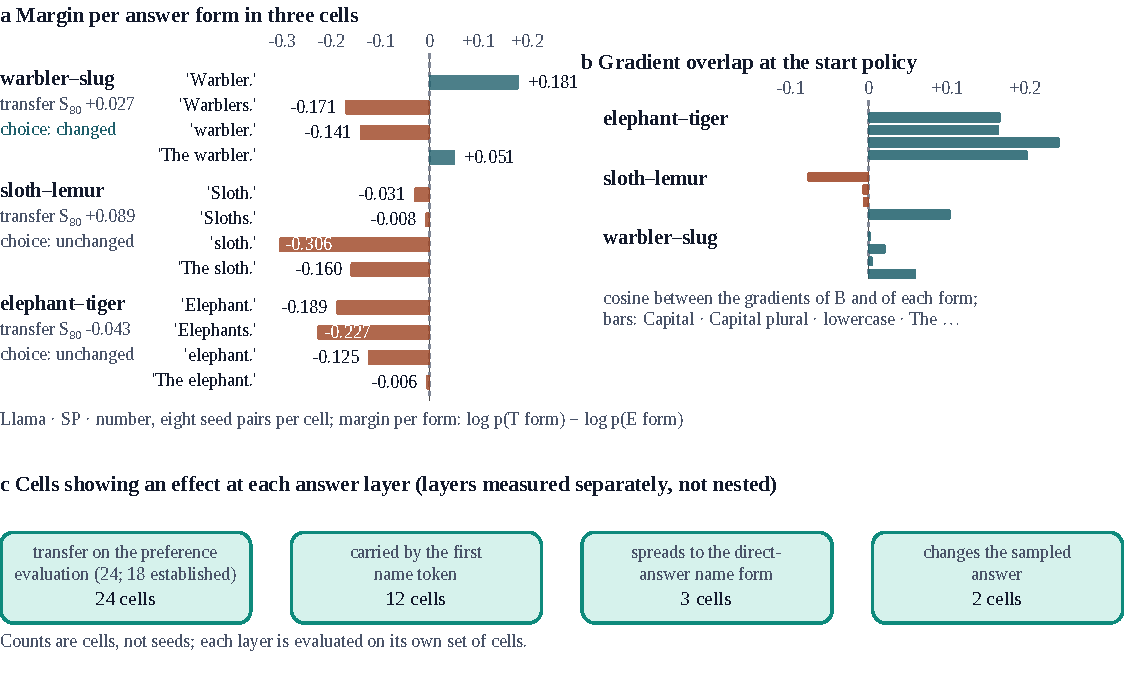
\includegraphics[width=\textwidth]{figs/f5.pdf}
\caption{\textbf{From transfer to a sampled answer.} \textbf{a}, Margin for each form the answer could take, in three cells. \textbf{b}, Overlap at the starting policy between the gradient of the preference margin and that of each form. \textbf{c}, Cells with an effect at each layer (one-sided $p < 0.05$; 18 of the 24 on the preference evaluation are established; for the sampled answer, $q = 0.28$ across the twelve sampled cells). Each layer is evaluated on its own set of cells.}
\label{fig:behaviour}
\end{figure*}



\paragraph{Which answer evaluation applies where} The forced-choice sign often reverses between presentation orders\cite{wang2024fair}, so it is unusable per seed pair, and the open-question evaluation is interpretable only while the two names' common component holds (Methods).

\paragraph{Why the open-question evaluation degenerates under same-model judges} A same-model judge's shared score is almost the student's own likelihood\cite{panickssery2024llm,wataoka2024selfpreference} ($r = 0.98$ for fine-tuned and $1.00$ for persona judges), so the shared reward sharpens the policy towards its modes\cite{huang2025sharpening} and lowers rare outputs such as an animal name as first word. Controlling base likelihood and length removes the anti-alignment entirely: this is not transfer acting against the trait, and it is why Llama behaviour is read from sampled answers.

\paragraph{Direct answers and echoes} We read choice from direct answers, whose first word is an animal name, and treat anything else as an echo (Methods); \st{Llama}{SP}{number}{elephant--tiger} shifts the order of mention ($p = 0.012$) without moving its direct-answer share, so counting echoes would credit it with a spurious choice effect. Among the 21 cells with a valid open-question evaluation, that evaluation moves only with established transfer, never without or against it (Supplementary Note~\ref{S-sn:behav}; every cell in Table~\ref{tab:main}).

\paragraph{The name form, not the size of transfer} \st{Llama}{SP}{number}{sloth--lemur} has twice the transfer of \st{Llama}{SP}{number}{warbler--slug} but no change in choice. Per-form margins (capitalized singular, capitalized plural, lowercase, ``The sloth.'') resolve this (Fig.~\ref{fig:behaviour}a): in warbler--slug the transfer reaches the capitalized singular, the form a direct answer uses (seven of eight seed pairs); in sloth--lemur it does not, and the lowercase form moves the other way.

The sign of this spread follows the start-policy overlap between the gradient of the preference margin and that of each direct-answer form (Fig.~\ref{fig:behaviour}b). Replayed at the start policy, the recorded updates predict the sign of each form's change relative to $B$ in 11 of 12 form predictions at step 80, and \st{Llama}{FT}{syllable}{shrew--cuttlefish}, with a fine-tuned judge, matches all four signs. Overlap gives direction, not magnitude: the one cell whose choice changed has the smallest overlaps and the single sign failure (Supplementary Note~\ref{S-sn:behav}).

\paragraph{Transfer without an answer-level result} \st{Qwen}{FT}{syllable}{otter--beaver}, \st{Qwen}{SP}{syllable}{otter--beaver} and \st{Qwen}{FT}{number}{sloth--lemur} move in the judge's direction (two established, the third at one-sided significance only) without an established answer-level result: their answer evaluation has 3.7 to 8.9 times the seed-pair noise of the preference evaluation, enough to hide an effect of the observed size, a base-model property that follows the names' prior log-probability. The steps of Fig.~\ref{fig:behaviour}c count cells measured at each layer and are not nested: one of the two cells whose sampled choice changes is not among the 18 with established transfer.
